%-------------------------------------------------------------------------------
\section{Performance Results}
%-------------------------------------------------------------------------------
\label{sec:perf-results}

% How is the ASP based solver performing?

The \clingo{} solver performance given a logic program depends on a number of factors. First, the number of facts in a specific concretization. Second, the configuration and various optimization parameters passed to the solver.

The solving process consists of four stages: \emph{setup}, \emph{load}, \emph{ground}, and \emph{solve}. The first two are preliminary phases and the other two perform the actual solve. Specifically, the setup phase generates the facts for the given spec, whereas the load phase loads the main logic program (i.e., the rules of the software model) as a resource into the solver. The grounding phase is the first part of the actual solve, it turns the facts and first-order logic rules into propositional logic. Once we have a grounded program, we can run the last phase, which is the full solve in \clingo{}.

We instrumented the solving code such that we obtained time measurements for each of the phases and the total time for the whole process.

\subsection{System Setup}

All performance runs were executed on a single node each of the Quartz
and Lassen supercomputers at Lawrence Livermore National
Laboratory. Each node of Quartz is an Intel Haswell CPU with 128GB of
memory. Each node of Lassen is an IBM Power9 little-endian CPU with
256GB of memory. No hardware accellerators were used in any of our
testing. All code ran out of an NFS directory running NFSv3.

\subsection{Solve timings for all packages}

In this section we examine the solving times for all the packages. First, we focus on the relation between the solving times and the number of dependencies for each package.

For number of dependencies, we measured the number of possible
dependencies added to the solve, rather than the total dependencies in
the result, because it is a closer measure of the necessary work for
the solver. This leads to natural clustering in the number of
dependencies, as many simple dependencies lead to large numbers of
potential dependencies that dwarf other differences between specs.


\begin{figure*}[htb]

    \centering
    \subfloat[][Ground times]{
    \label{subfig:deps_quartz_load}
        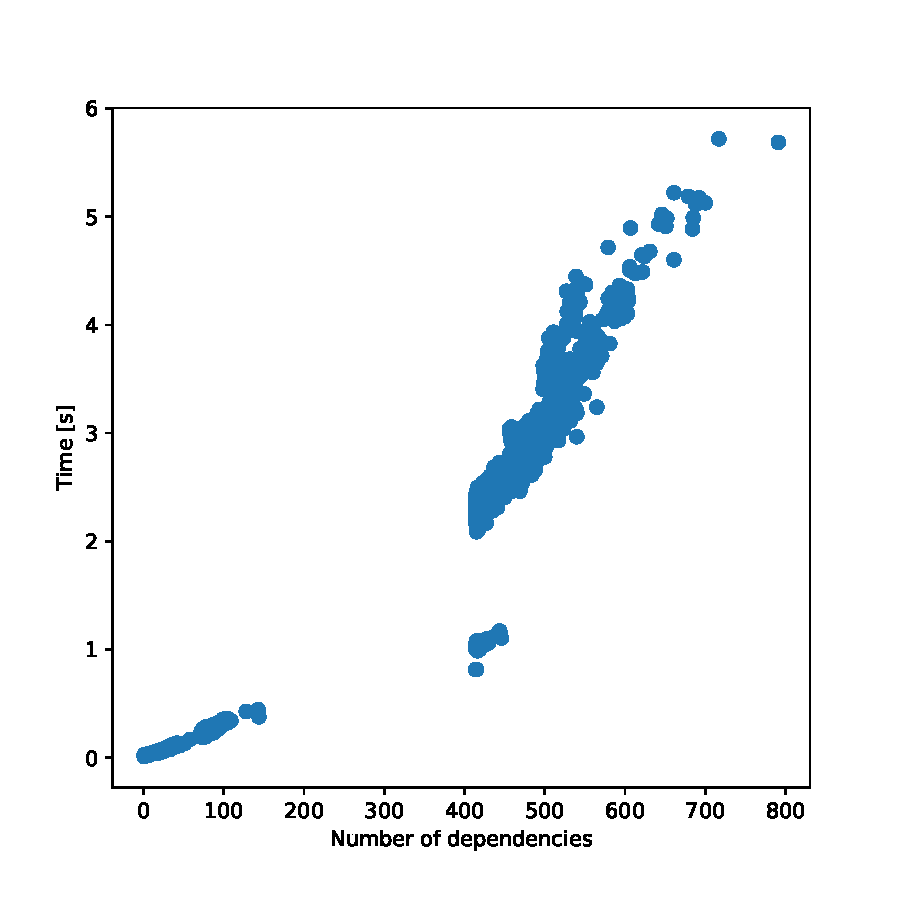
\includegraphics[width=0.32\textwidth]{figures/perf/deps_quartz_ground_fig.pdf}
    }\hfill%
    \subfloat[][Solve times]{
    \label{subfig:deps_quartz_solve}
        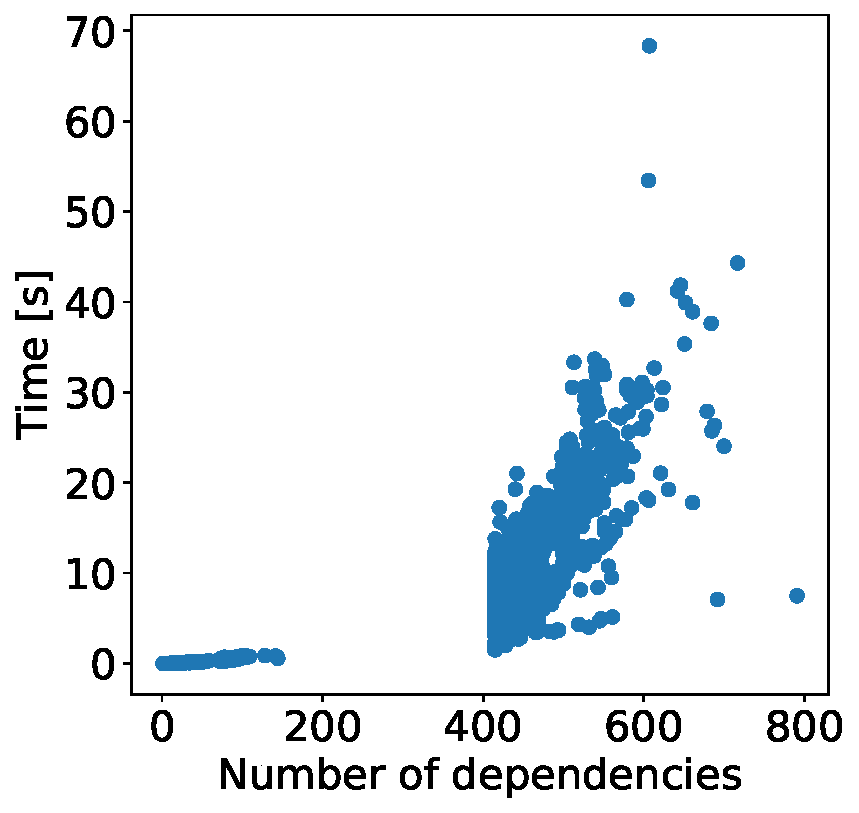
\includegraphics[width=0.32\textwidth]{figures/perf/deps_quartz_solve_fig.pdf}
    }\hfill%
    \subfloat[][Full solving times]{
    \label{subfig:deps_quartz_full}
        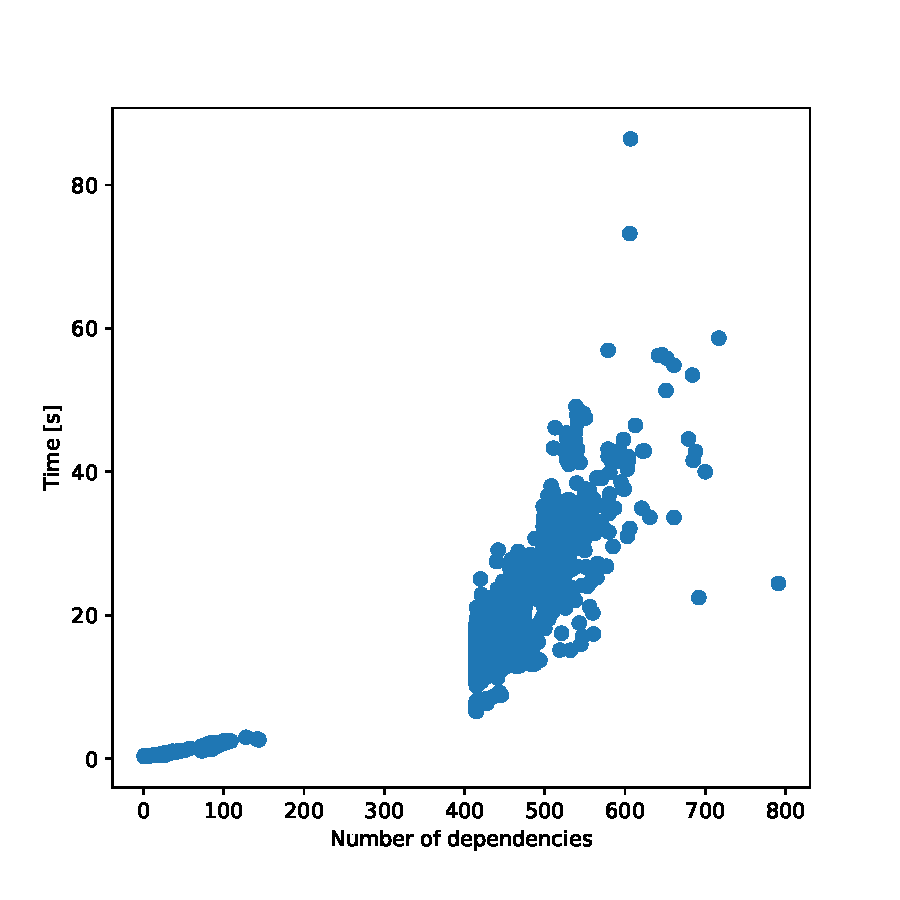
\includegraphics[width=0.32\textwidth]{figures/perf/deps_quartz_total_fig.pdf}
    }
    \caption{Solve times vs. number of dependent packages across all packages on the Quartz machine.}
    \label{fig:deps_quartz}

\end{figure*}



\begin{figure*}[htb]

    \centering
    \subfloat[][Ground times]{
    \label{subfig:deps_lassen_load}
        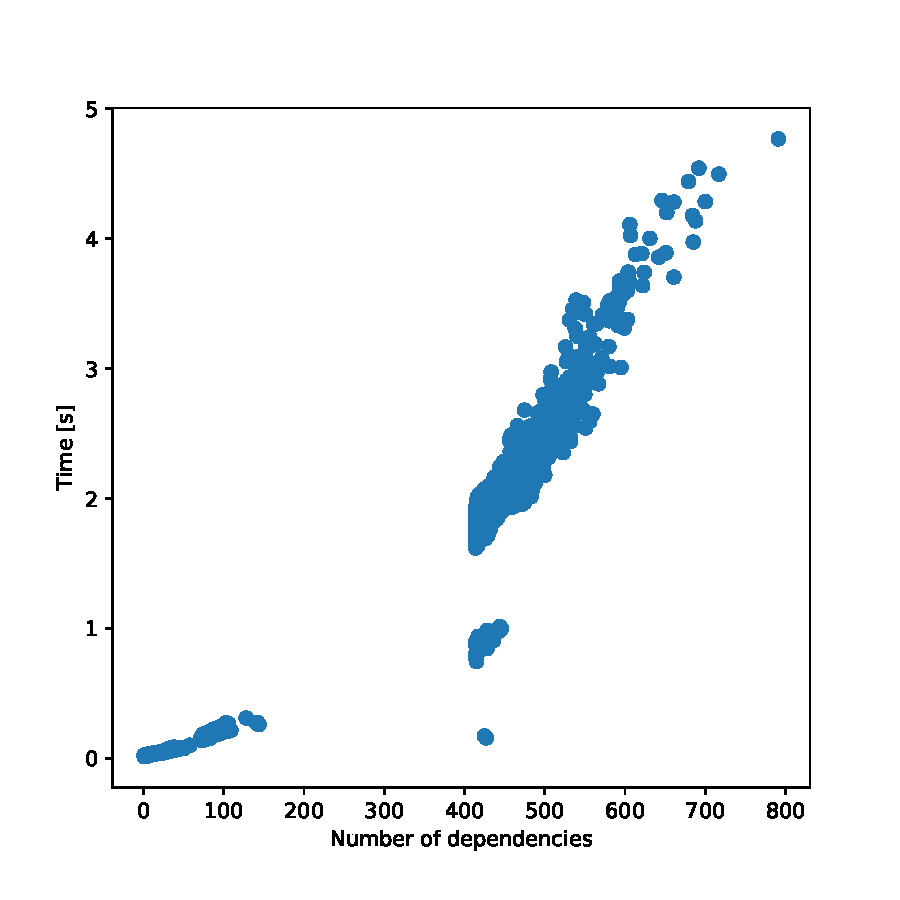
\includegraphics[width=\perfsubfigwidth\textwidth]{figures/perf/deps_lassen_ground_fig.pdf}
    }\hfill%
    \subfloat[][Solve times]{
    \label{subfig:deps_lassen_solve}
        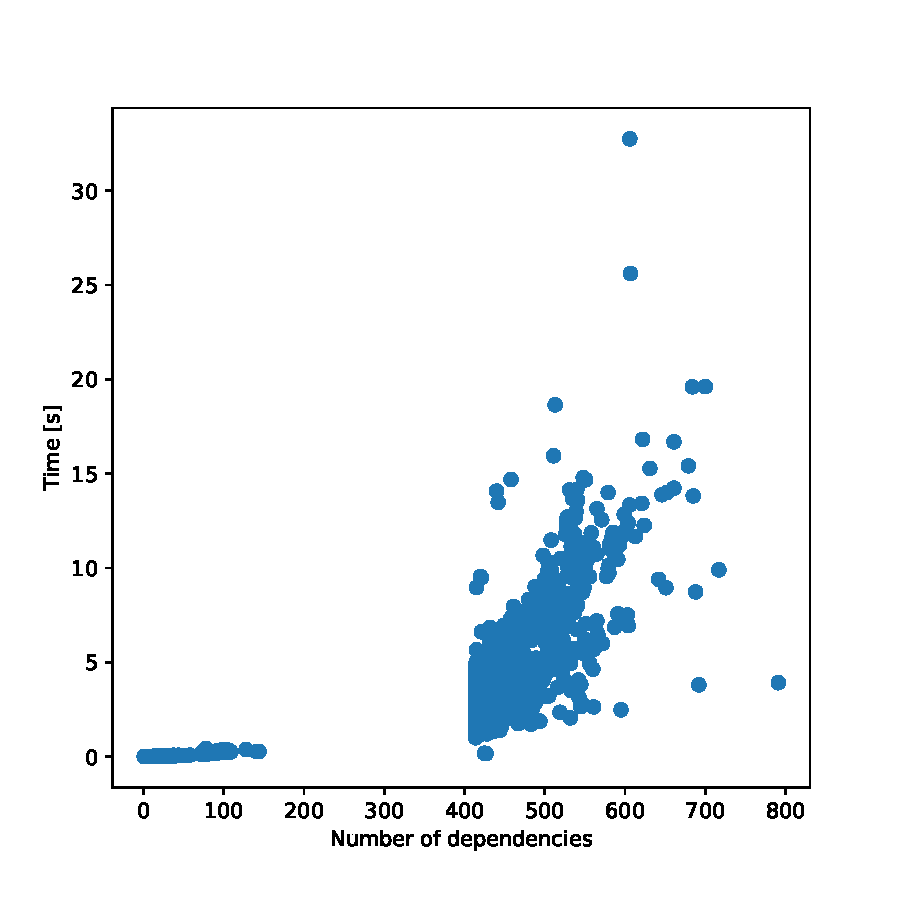
\includegraphics[width=\perfsubfigwidth\textwidth]{figures/perf/deps_lassen_solve_fig.pdf}
    }\hfill%
    \subfloat[][Full solving times]{
    \label{subfig:deps_lassen_full}
        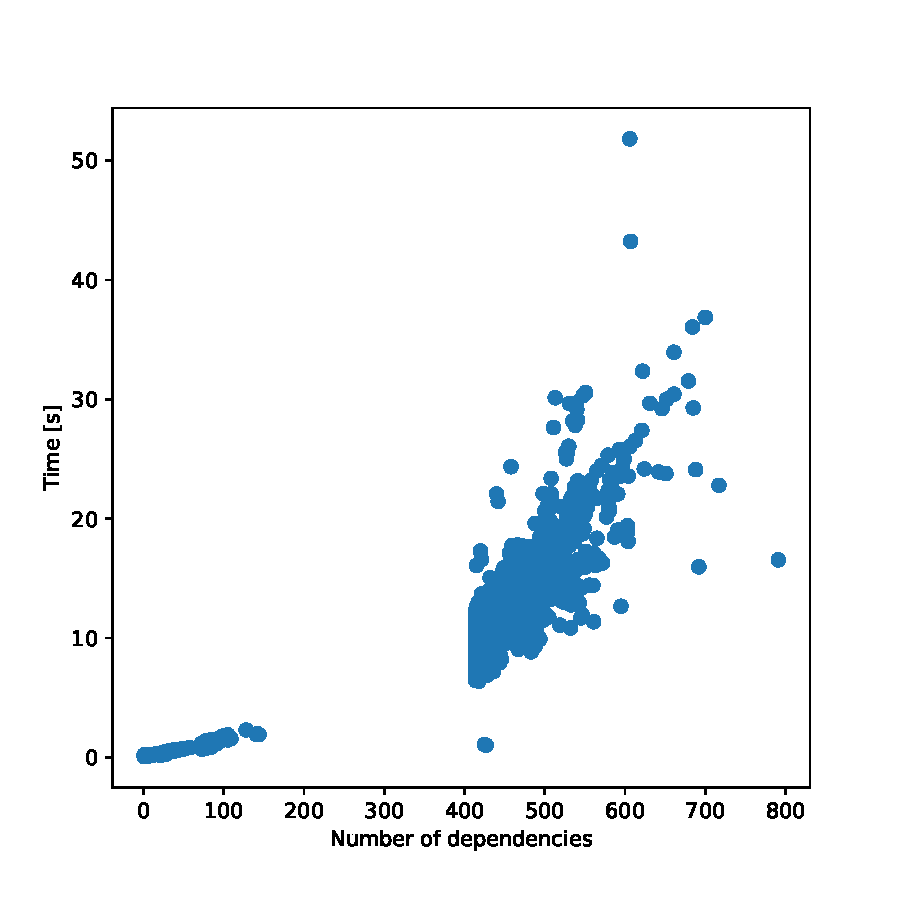
\includegraphics[width=\perfsubfigwidth\textwidth]{figures/perf/deps_lassen_total_fig.pdf}
    }
    \caption{Solve times vs. number of dependent packages across all packages on the Lassen machine.}
    \label{fig:deps_lassen}

\end{figure*}


Figures~\ref{fig:deps_quartz} and~\ref{fig:deps_lassen} show the grounding, solve, and full solving (i.e., involving all the stages) times for all the packages on Quartz and Lassen, respectively~\cite{llnl:hpc}. Quartz is an Intel-based 3.3 Petaflop cluster at Lawrence Livermore National Laboratory (LLNL). Each node comprises of two Intel Xeon E5-2695 v4 processors and 128GB of memory. The Lassen machine at LLNL is a smaller variant of Sierra, a 125 Petaflop machine. Each node on Lassen has two IBM POWER9 processors and four NVIDIA Tesla V100 (Volta) GPUs, as well as 256GB of memory. Load times, as one would expect, were not affected by the number of packages. Also, the setup times are the same order of magnitude as ground times and do not depend on \clingo{}'s performance so they were ommitted in favor of showing times that are directly dependent on \clingo{}. We used the \clingo{}'s "tweety" configuration and "usc,one" optimization strategy for running the solving process. Further below we explore the differences in solving times between these different strategies.

We can see from the figures that the time increases as the number of possible package dependencies increases. This is because increased number of possible dependencies leads to a larger number of facts and a bigger logic program overall. We measure possible dependencies rather than actual dependencies of the result because possible dependencies better measure the size of the problem space. In particular, when many packages can provide a virtual dependency like the Message Passing Interface (MPI), much of the potential solve space is not present in the final result when a single MPI implementation is chosen.

Figures~\ref{fig:deps_quartz} and~\ref{fig:deps_lassen} also show that there are two major clusters in the execution times. The clusters are separated by a gap in the possible dependencies. One cluster contains packages with less than 200 possible dependencies, whereas, the other major cluster contains packages with more than 400 possible dependencies. This natural clustering occurs because some low-level dependencies have options that can trigger huge potential dependency trees, and the gap is between packages that can include those dependencies and those that cannot.

% TODO: Can we confirm this?? My explanation above is slightly vague -- GBB
% The gap occurs because of dependency on \emph{cmake}, which itself depends cumulatively on more than 400 packages.

Besides dependencies another set of factors that influences the execution times are \clingo{} parameters. Specifically, \clingo{} defines six configuration presets: \emph{frumpy}, \emph{jumpy}, \emph{tweety}, \emph{trendy}, \emph{crafty}, and \emph{handy}. Each preset sets numerous low level parameters that control different aspects of the solver. In our performance study, we specifically focus on three configurations: \emph{tweety} -- geared towards typical ASP programs, \emph{trendy} -- geared towards industrial problems, and \emph{handy} -- geared towards large problems.


\begin{figure*}[htb]

    \centering
    \subfloat[][Ground times]{
    \label{subfig:cdf_quartz_ground}
        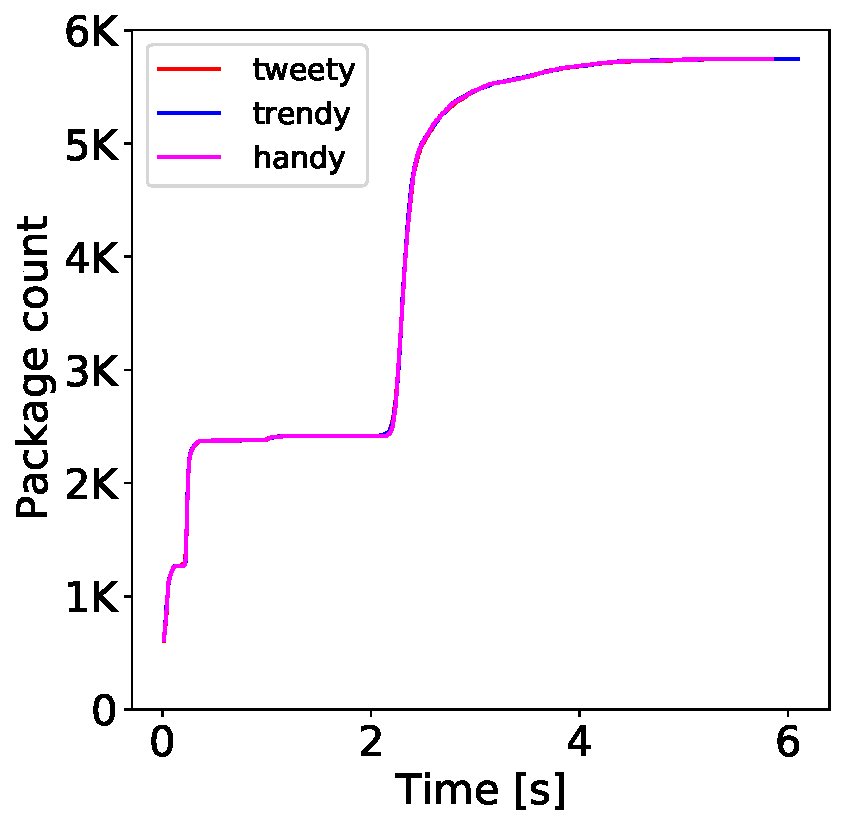
\includegraphics[width=\perfsubfigwidth\textwidth]{figures/perf/cdf_quartz_ground_fig.pdf}
    }\hfill%
    \subfloat[][Solve times]{
    \label{subfig:cdf_quartz_solve}
        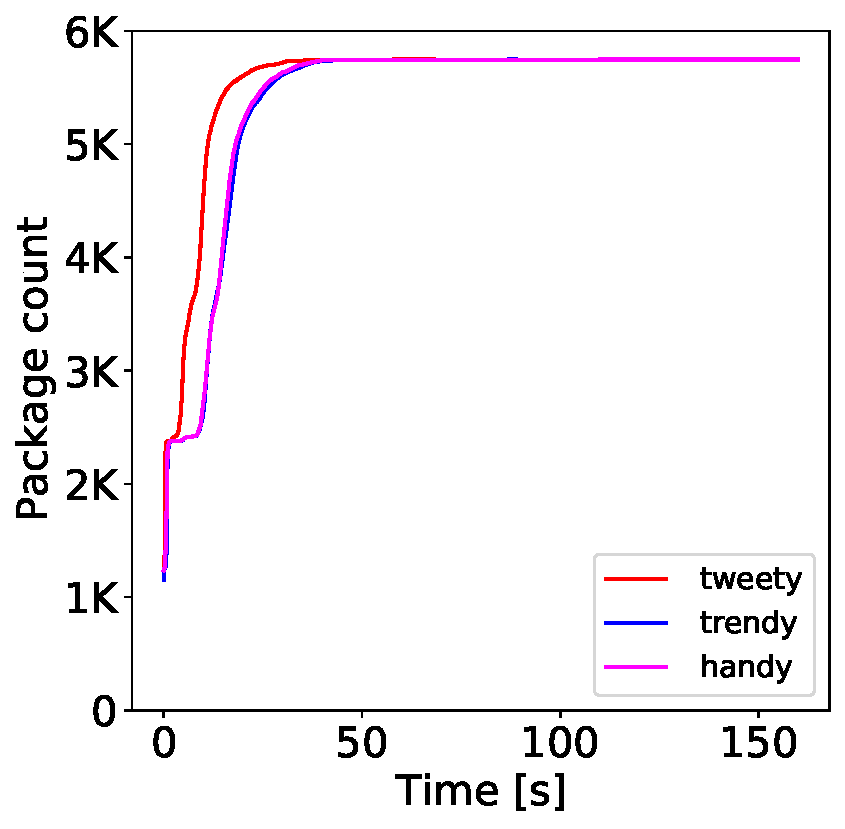
\includegraphics[width=\perfsubfigwidth\textwidth]{figures/perf/cdf_quartz_solve_fig.pdf}
    }\hfill%
    \subfloat[][Full solving times]{
    \label{subfig:cdf_quartz_full}
        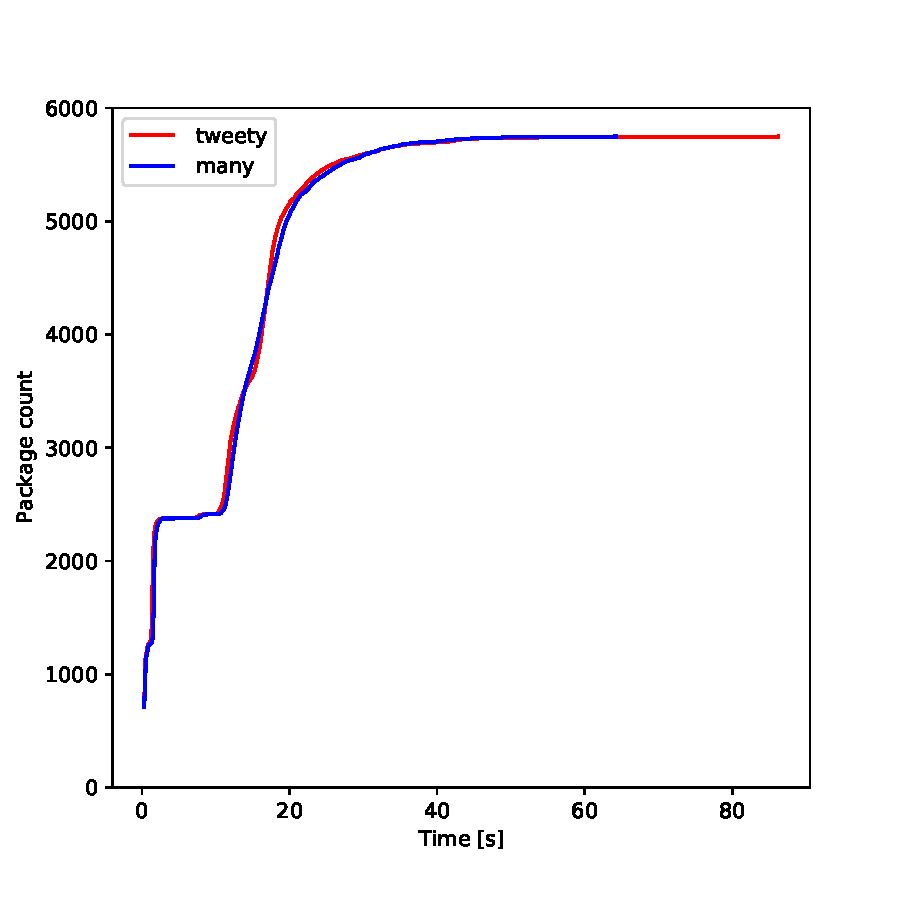
\includegraphics[width=\perfsubfigwidth\textwidth]{figures/perf/cdf_quartz_total_fig.pdf}
    }
    \caption{Cumulative distribution of solve times across all packages on the Quartz machine.}
    \label{fig:cdf_quartz}

\end{figure*}



\begin{figure*}[htb]

    \centering
    \subfloat[][Load times]{
    \label{subfig:cdf_lassen_load}
        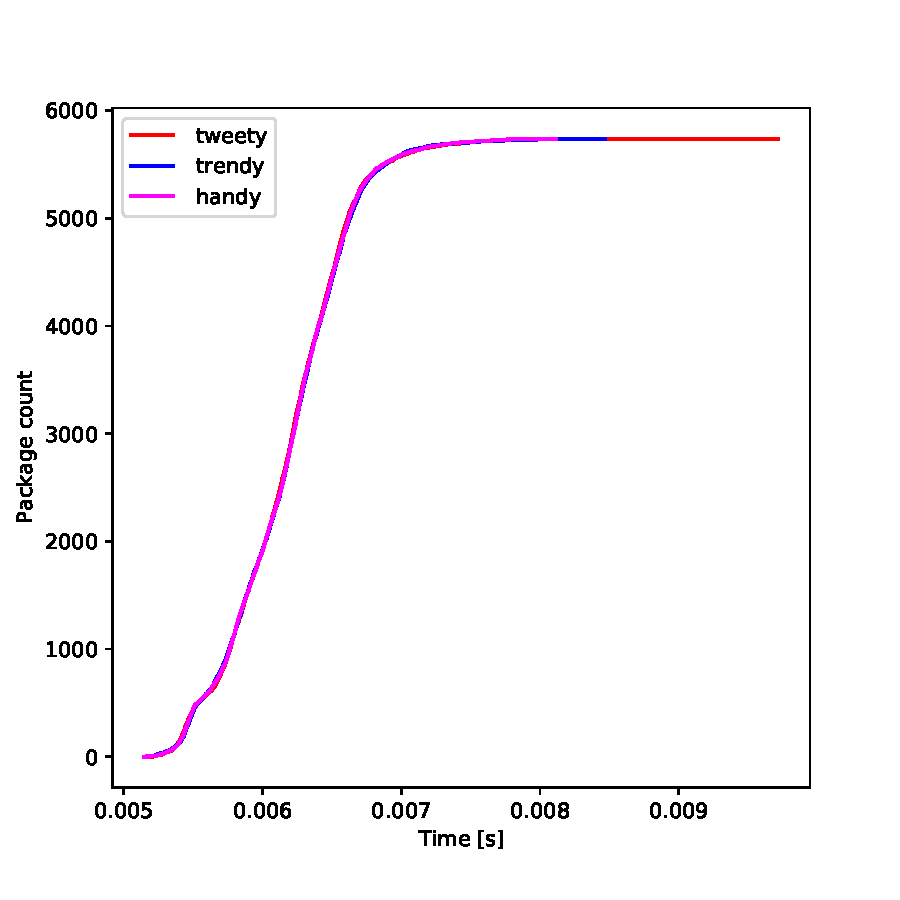
\includegraphics[width=0.32\textwidth]{figures/perf/cdf_lassen_load_fig.pdf}
    }\hfill%
    \subfloat[][Solve times]{
    \label{subfig:cdf_lassen_solve}
        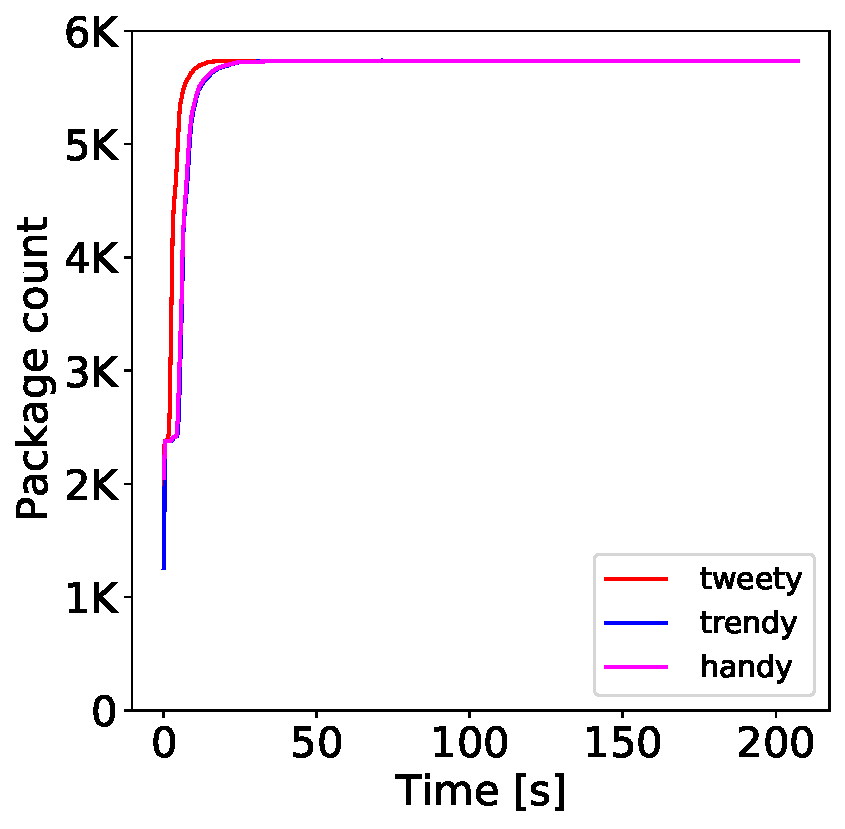
\includegraphics[width=0.32\textwidth]{figures/perf/cdf_lassen_solve_fig.pdf}
    }\hfill%
    \subfloat[][Full solving times]{
    \label{subfig:cdf_lassen_full}
        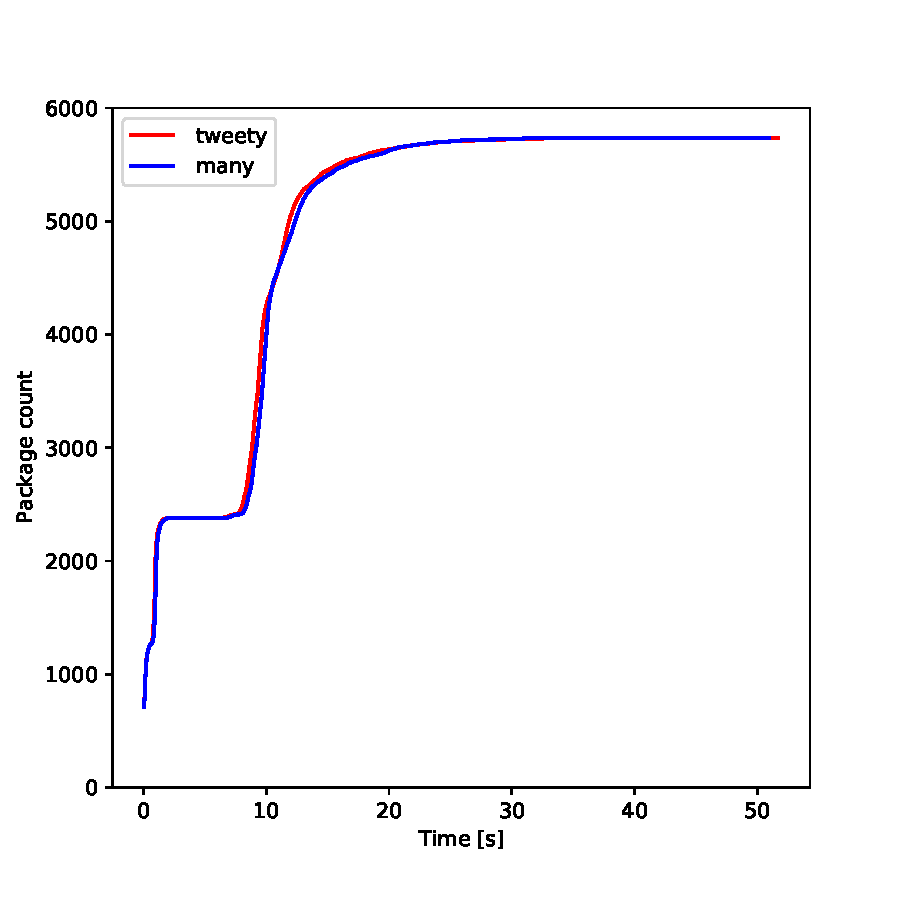
\includegraphics[width=0.32\textwidth]{figures/perf/cdf_lassen_total_fig.pdf}
    }
    \caption{Cumulative distribution of solve times across all packages on the Lassen machine.}
    \label{fig:cdf_quartz}

\end{figure*}


Figures~\ref{fig:cdf_quartz} and~\ref{fig:cdf_lassen} show the cumulative distribution of the solve times under \emph{tweety}, \emph{trendy}, and \emph{handy} configurations on Quartz and Lassen machines, respectively. The vast majority of packages are fully solved in under 25 seconds on both machines. We can also see that there is no difference in ground times between the different configurations. This suggests that most low level parameters that are tweaked by each configuration control the actual solving phase. The figures cleary indicate that \emph{tweety} performs better than the other configurations we benchmarked. This is, therefore, the default configuration used in the concretization process.

% - other properties?
% - --single-shot vs. no single-shot?
% - different tactics?

\subsection{Solve timings for all packages with reuse}

In this subsection, we examine the performance of the solver with the \emph{reuse} flag switched on. As described in Section~\ref{sec:reuse}, reusing packages in a buildcache increases the number of facts proportionally to the number of cached packages.

We specifically focus on the packages in the ECP Extreme-scale Scientific Software Stack (E4S) project~\cite{e4s}. It is a community effort to provide open source software packages for developing, deploying, and running scientific applications on HPC platforms. There are just under 600 packages in E4S, but the buildcache of the project targets different architectures, operating systems, and compilers, thereby totaling over 60K pre-compiled packages (hash signatures). We divided the buildcache into 4 groups: full buildcache (63099 packages), buildcache restricted to the \texttt{ppc64le} architecture (27160 packages), buildcache restricted to the \texttt{rhel7} OS (15255 packages), and buildcache restricted to both \texttt{ppc64le} architecture and the \texttt{rhel7} OS (6804 packages). Benchmarking across an increasing size of the buildcache provides us with a better understanding of the impact of the package resuse functionality.


\begin{figure*}[htb]

    \centering
    \subfloat[][Setup times]{
    \label{subfig:cdf_e4s_quartz_load}
        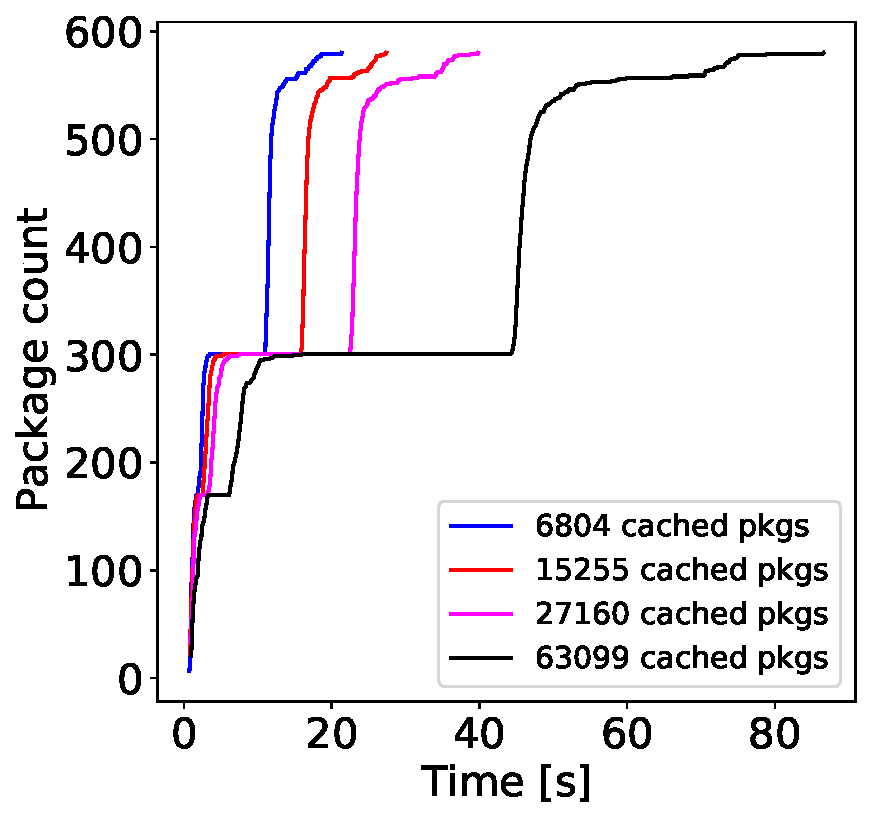
\includegraphics[width=\perfsubfigwidth\textwidth]{figures/perf/cdf_e4s_cache_quartz_setup_fig.pdf}
    }\hfill%
    \subfloat[][Solve times]{
    \label{subfig:cdf_e4s_quartz_solve}
        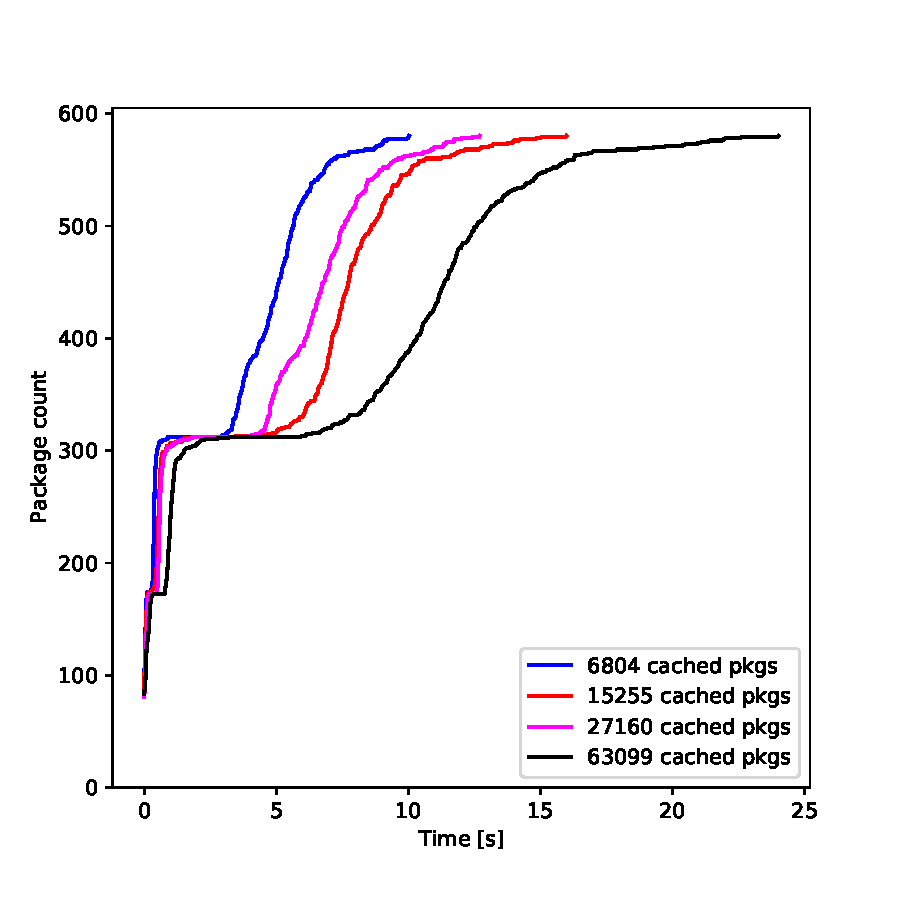
\includegraphics[width=\perfsubfigwidth\textwidth]{figures/perf/cdf_e4s_cache_quartz_solve_fig.pdf}
    }\hfill%
    \subfloat[][Total solver times]{
    \label{subfig:cdf_e4s_quartz_full}
        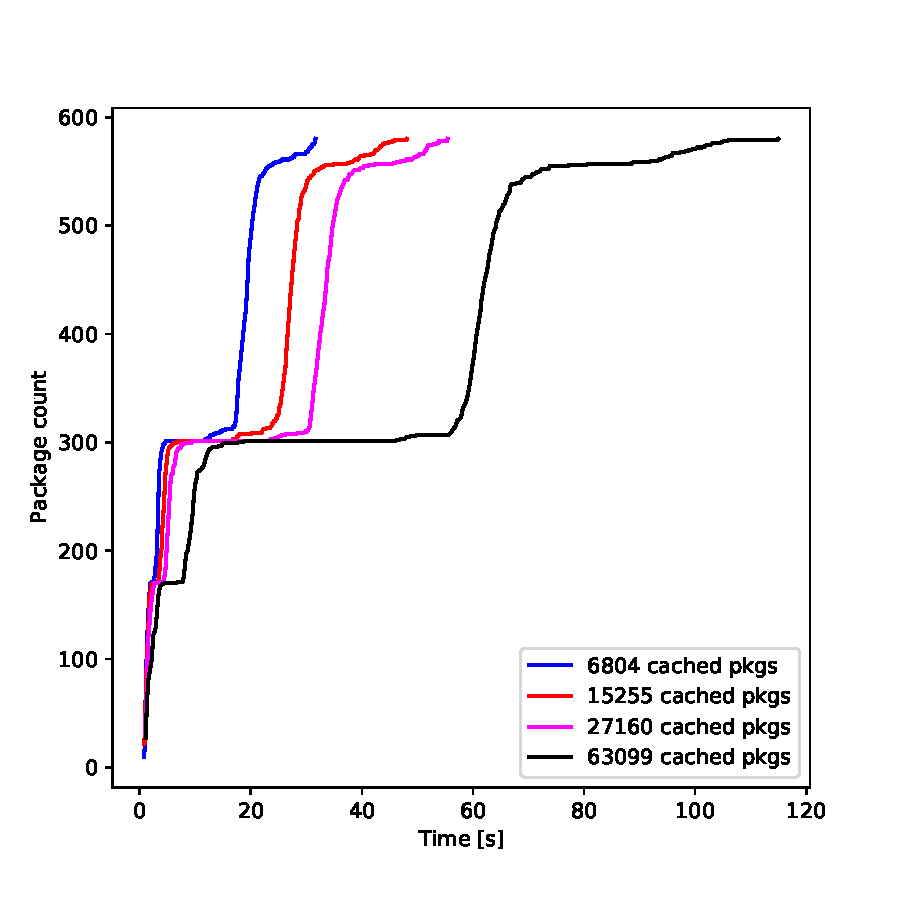
\includegraphics[width=\perfsubfigwidth\textwidth]{figures/perf/cdf_e4s_cache_quartz_total_fig.pdf}
    }
    \caption{Cumulative distribution of solve times for different cache sizes across all E4S packages on the Quartz machine.}
    \label{fig:cdf_e4s_quartz}

\end{figure*}



\begin{figure*}[htb]

    \centering
    \subfloat[][Setup times]{
    \label{subfig:cdf_e4s_lassen_load}
        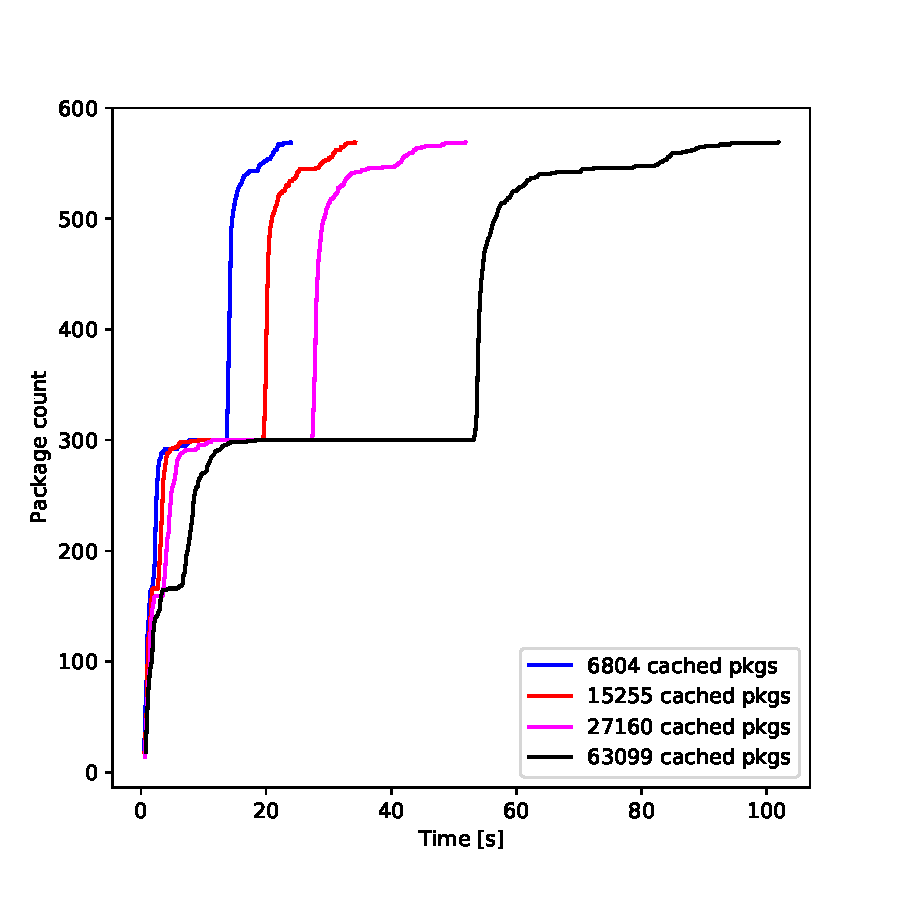
\includegraphics[width=0.32\textwidth]{figures/perf/cdf_e4s_cache_lassen_setup_fig.pdf}
    }\hfill%
    \subfloat[][Solve times]{
    \label{subfig:cdf_e4s_lassen_solve}
        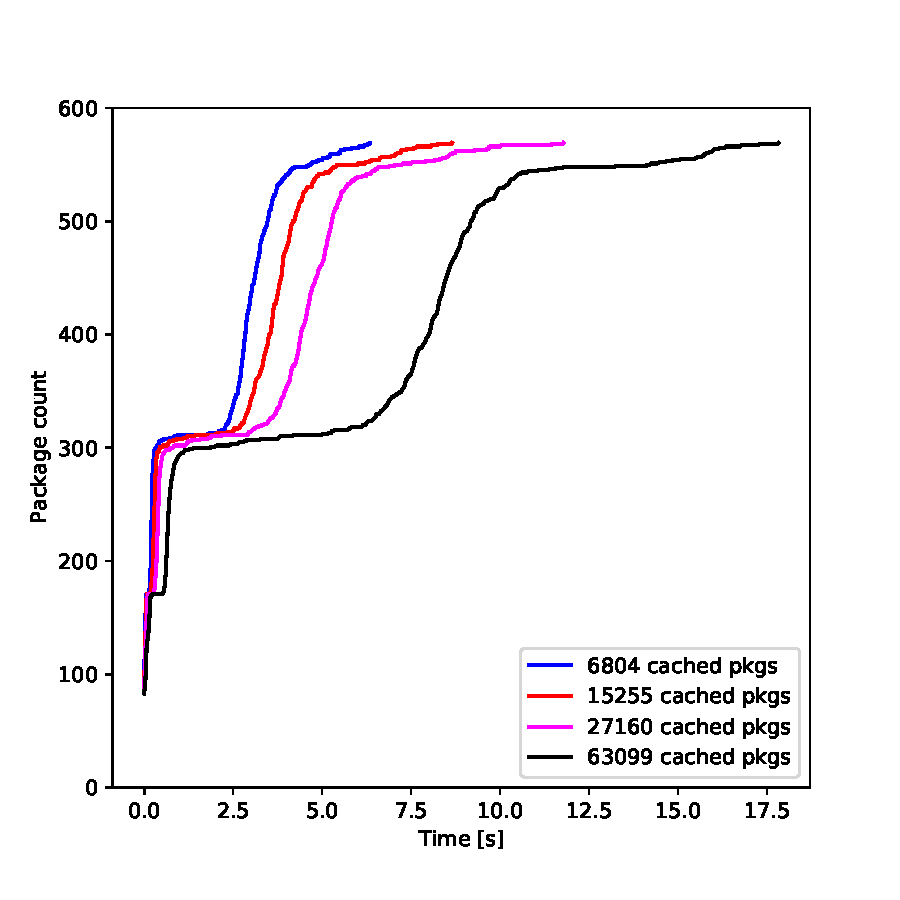
\includegraphics[width=0.32\textwidth]{figures/perf/cdf_e4s_cache_lassen_solve_fig.pdf}
    }\hfill%
    \subfloat[][Total solver times]{
    \label{subfig:cdf_e4s_lassen_full}
        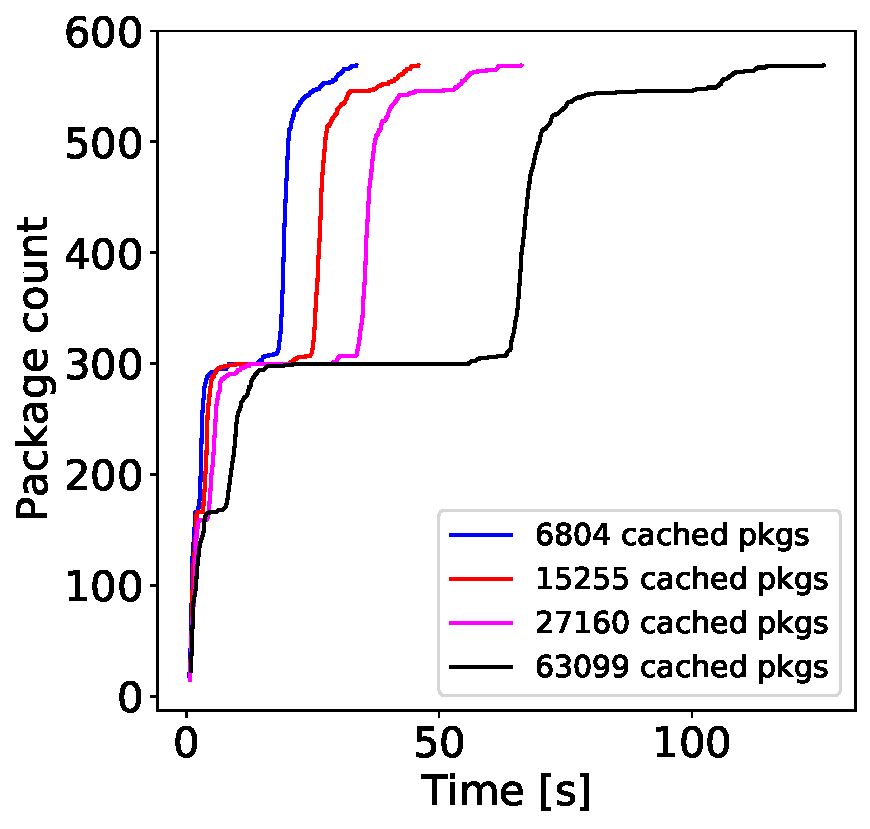
\includegraphics[width=0.32\textwidth]{figures/perf/cdf_e4s_cache_lassen_total_fig.pdf}
    }
    \caption{Cumulative distribution of solve times for different cache sizes across all E4S packages on the Lassen machine.}
    \label{fig:cdf_e4s_lassen}

\end{figure*}


Figures~\ref{fig:cdf_e4s_quartz} and~\ref{fig:cdf_e4s_lassen} show the cumulative distribution of the solve times of the E4S packages with increasing buildcache on Quartz and Lassen, respectively. We first observe that the setup times are generally higher than the actual solve times, even for smaller buildcaches. This happens because when we reuse packages we need to encode much more facts than usual, which are facts representing the dependencies. The figures also show that there is a significant jump in the solve times for the biggest buildcache. The majority of this jump occurs in the setup phase, as shown in the figures, suggesting that the runtime is being dominated by the serial process of generating facts for the solver, rather than exponential explosion in the solver. This suggests positive outcomes for future work improving performance in this area.
